% Chapter Template

\chapter{Supervised Validation}%
\label{chap:supervised_validation}

The approaches we have presented so far work fully unsupervised.
Given two collections of definitions, we have tried to retrieve the definition(s) that represented the same meaning.
However, given the moderately sized data in our hands we have accepted as \enquote{golden}, we studied the feasibility of training an encoder~\cite{sutskever_sequence_2014}, where the objective is to learn whether the pair of definitions entail the same sense across languages.

Recurrent Neural Network (RNN) architectures improve upon the prototypical neural network model by introducing a \emph{memory} for the connections in the network~\cite{rumelhart_learning_1986}.
By updating the hidden unit over time using the output of the previous time step, the model can \emph{remember} features of the input signal for later inputs.
% TODO figure here
%RNN seemed fitting for our case given their success on tasks that require a model to \emph{remember} previous signals over a long sequence of inputs\cite{gers_lstm_2001,jean_using_2014}.
One particular architecture of RNNs propsed by \textcite{hochreiter_long_1997} is \emph{long short-term memory} (LSTM).
LSTM models have been successful on language modelling tasks~\cite{sutskever_sequence_2014}, handwriting recognition~\cite{graves_unconstrained_2008,graves_novel_2009} and machine translation with a focus on rare words~\cite{luong_addressing_2014} to name a few.
Highlight of these results are that LSTM has an advantage on tasks that require contextual information to persist over long periods of time~\cite{graves_long_2012}.
Furthermore, LSTMs do not require fixed input vectors, which is a necessity for us since our definition pairs do not have to be the same size.

\subsection{Vanishing Gradient Problem}%
\label{sub:vanishing_gradient_problem}

LSTM is borne out of the need to address the \emph{vanishing gradient problem}~\cite{hochreiter_long_1997, bengio_learning_1994}.
On the original publication by \textcite{hochreiter_long_1997}, a crucial shortcoming of RNNs have been identified as their slow rate of training which may not converge in the end at all.
Independently, \textcite{bengio_learning_1994} suggested that the problem stems from the choice between the conservation of the previous inputs versus resisting against the noise they accumulate.
Figure~\ref{fig:vanishing_gradients}, adapted from \textcite{graves_long_2012} illustrates the problem using shades as the influence of input over neural network units.

\begin{figure}[htbp]
    \centering
    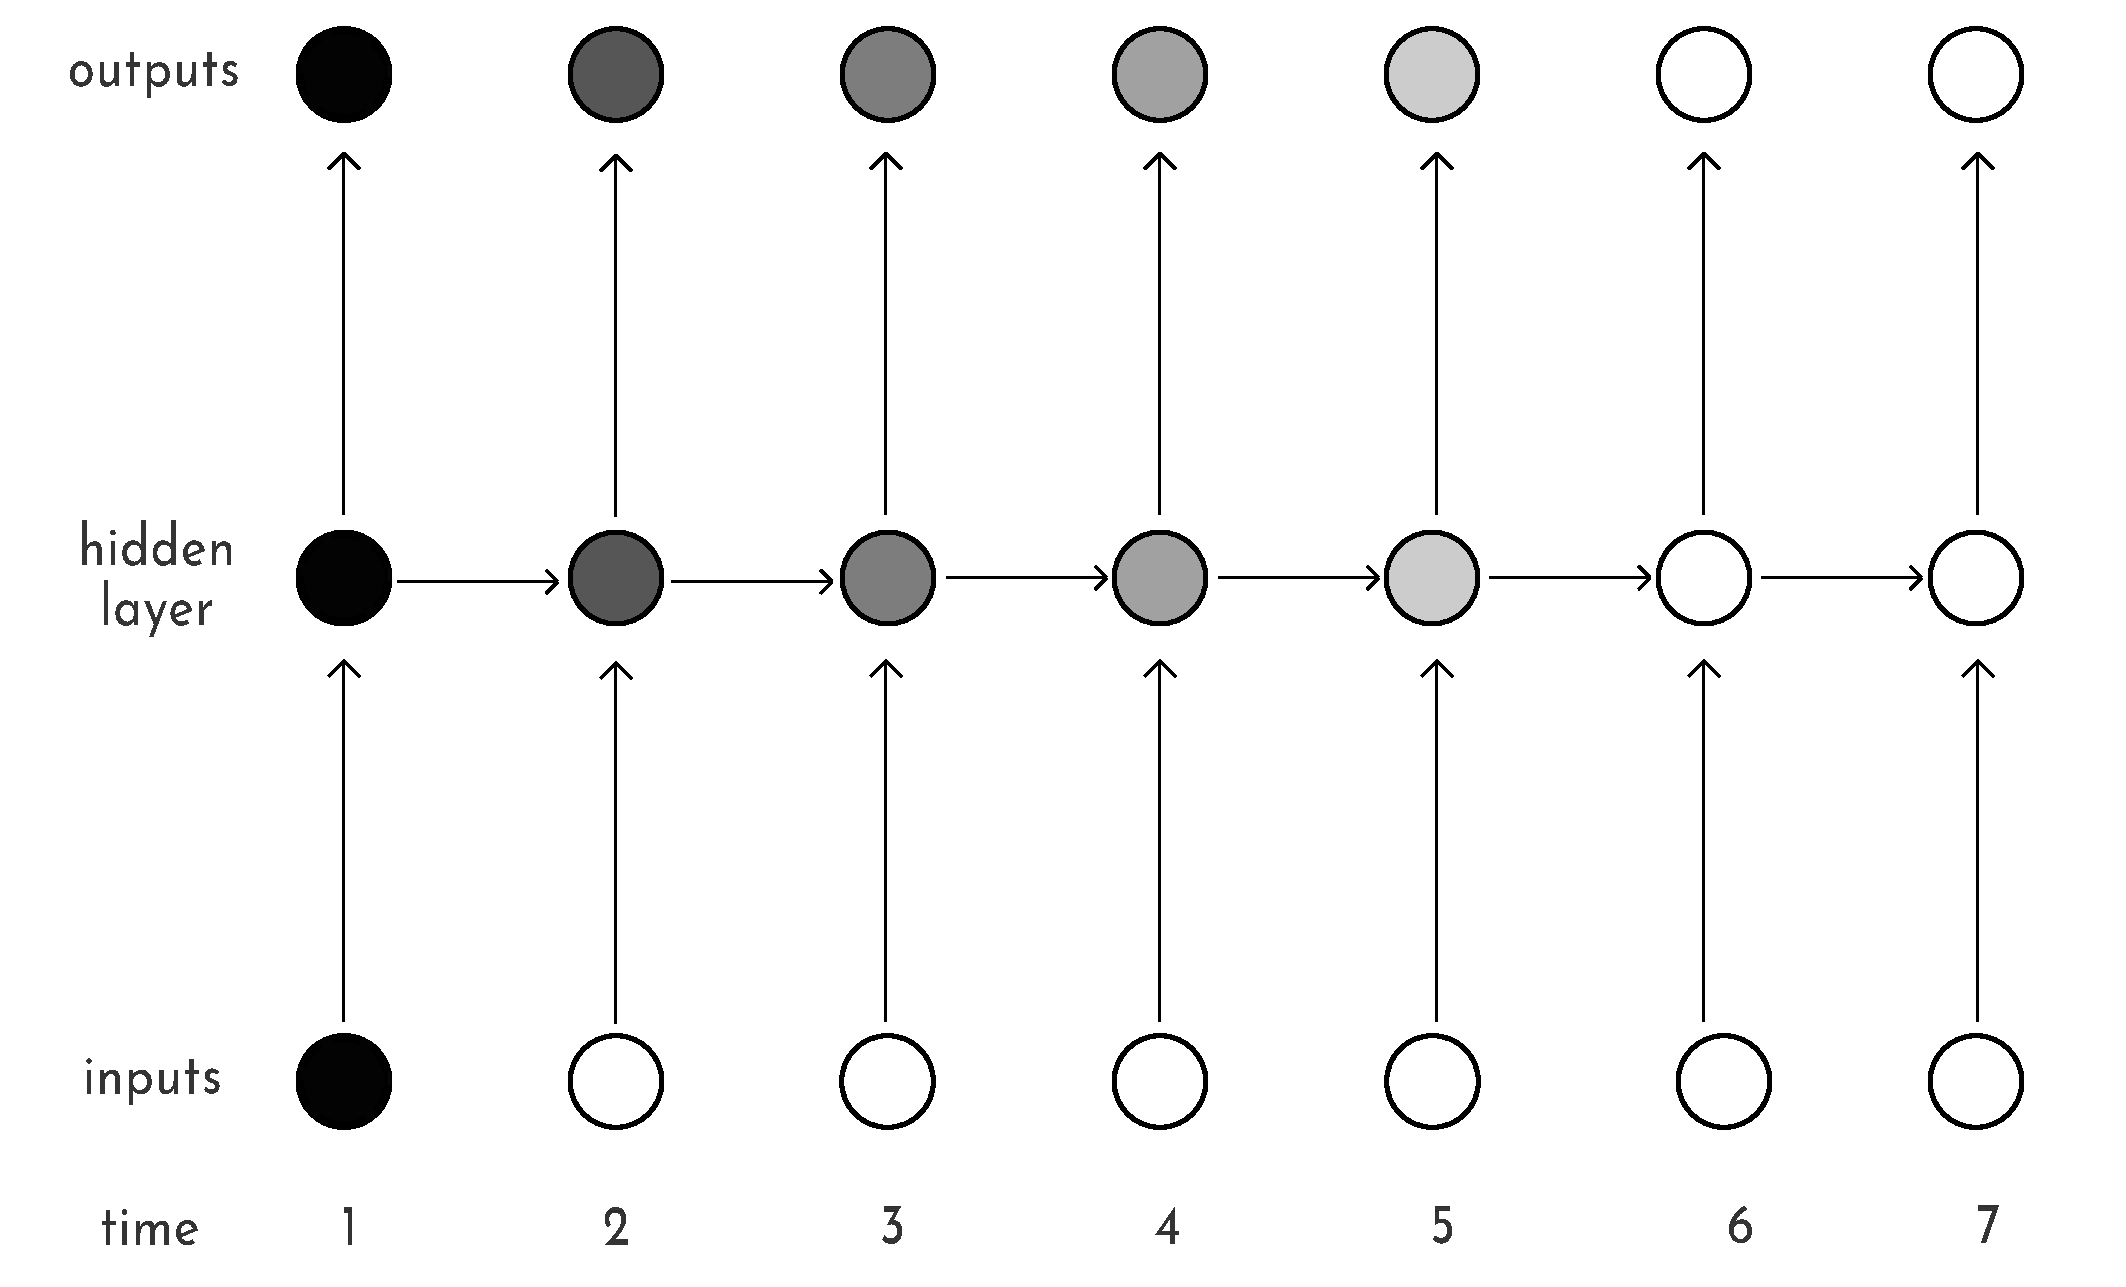
\includegraphics[page=1,width=\textwidth]{Figures/outputs_hiddenlayer.pdf}
    \caption{Graphical representation of vanishing gradient problem where the shades of the nodes represent the influence of the input signal, adapted from Figure 4.1 of \textcite{graves_long_2012}}%
    \label{fig:vanishing_gradients}
\end{figure}

% Input -> will cell learn/change
% Forget -> will cell reset
% Output -> Will cell propagate

%The issue is related to a natural disadvantage of Recurrent Neural Networks (RNN).
As the input signal traverses the units of an RNN, it either diminishes or blows up~\cite{graves_long_2012}.
A long line of solutions were proposed such as decomposing structures so that only unexpected ones can be relevant.
% TODO give more solutions here

\subsection{Long Short-Term Memory}%
\label{sub:lstm}

LSTM is the solution highlighted by \textcite{graves_long_2012} as a recurrent neural network model that can work over temporally distant input signals while preserving their influence or diminishing their noise.
The centrepiece idea is to use a \emph{constant error carousel}, special cells that enforce a constant error flow.
In the original paper, this complex unit is named \emph{memory cell}~\cite{hochreiter_long_1997}.
Using an \emph{input gate}, the cell is updated if the current input is relevant and using an \emph{output gate}, the unit will not update other cells if the current input is not relevant.
A simplified overview of the suggested model is presented in Figure~\ref{fig:simple_lstm}.

\begin{figure}[htbp]
    \centering
    \incfig{simple_lstm}
    \caption{Simplified long short-term memory cell architecture}%
    \label{fig:simple_lstm}
\end{figure}
% We kept forward pass and backprop equations out because no time and out of scope hopefully

Multiple arrows denote input from current time frame and recurrent connections.
$\odot$ symbol denotes multiplication.
By weighing the input and output gates between 0 and 1, the impact of the current input can be adjusted.
Overall, input gate controls how much cell will learn and output gate controls how much the cell will propagate.
Figure~\ref{fig:lstm_preserves} adapted from \textcite{graves_long_2012} illustrates how the LSTMs operate against vanishing gradient.

\begin{figure}[htbp]
    \centering
    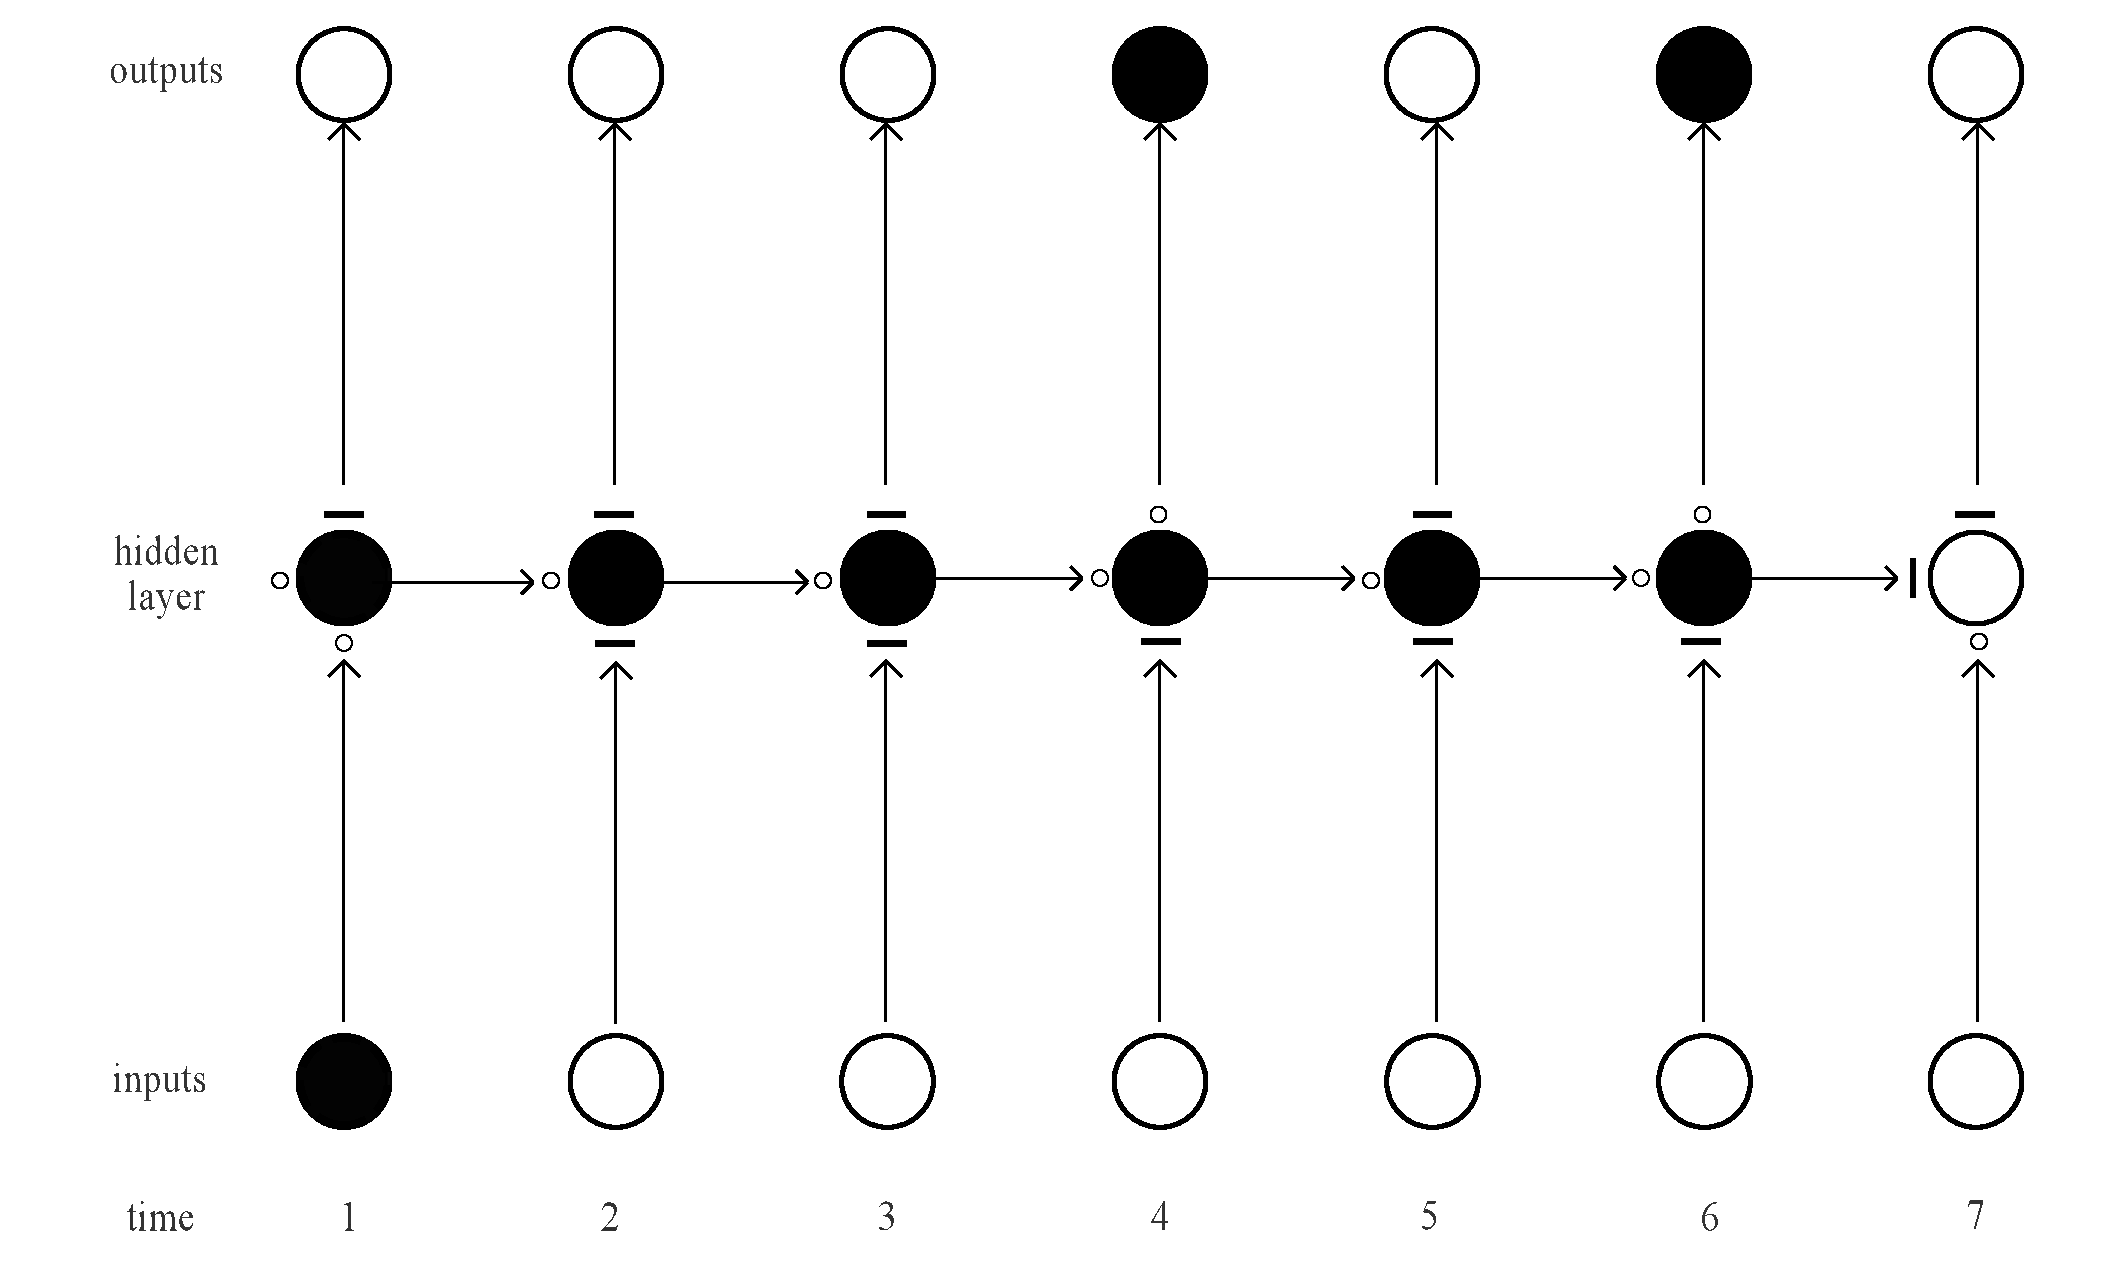
\includegraphics[page=1,width=\textwidth]{Figures/outputs_hiddenlayer2.pdf}
    \caption{Preserving the input signal through blocking (-) or allowing (O) the input signal, adapted from Figure 4.4 of \textcite{graves_long_2012}}%
    \label{fig:lstm_preserves}
\end{figure}

% forget gate
Two gates on top of the cell structure model got extended with a third \emph{forget gate} by \textcite{gers_learning_2000}.
The aim was to handle input sequences that are not segmented in a predictable manner.
The proposed forget gate is implemented to \emph{reset} the cell.
When a cell state got irrelevant due to a change in problem domain, forget gate gradually resets the cell state instead of erroneous activations from the input gate.

% peephole connections
Another extension came in the form of \emph{peephole connections} by \textcite{gers_learning_2003}.
By allowing internal gates to inspect the cell state, they have shown improvements on non-linear tasks.

% \textcite{pascanu_difficulty_2012}

The finalized model with input, forget and output gates as well as the internal peephole connections was debuted in \textcite{graves_framewise_2005}.
In their expansive study comparing 8 LSTM variants over 15 years of CPU time, \textcite{greff_lstm_2017} named this model the \enquote{vanilla LSTM}.
This particular form of LSTM is commonly used~\cite{sutskever_sequence_2014}.
The real valued vectors are denoted alongside their update time step ${(\cdot)}_t$ such that $t \in {1, \dots, T}$.
Updates are performed on the input gate $i_t$, memory cell $c_t$, forget gate $f_t$ and output gate $o_t$.
We show the updates over weight matrices $W_i, W_f, W_c$ and $W_o$ via the use of recurrent weights $R_i, R_f, R_c$ and $R_o$ and bias vectors $b_i, b_f, b_c$ and $b_o$.
Peephole connections are shown using $p_{\cdot}$ for input, forget and output gates as $p_{i}, p_{f}$ and $p_{o}$ respectively.
Finally, the input is a sequence of data in the form of $(x_1, x_2, \dots, x_T)$ and the model outputs real valued vector $y_{t}$ at the time step $t$.

\begin{equation}
    i^{t} = \sigma\left(W_{i}x^{t} + R_{i}y^{t-1} + p_{i} \odot c^{t-1} + b_{i}\right)
\end{equation}

\begin{equation}
    f^{t} = \sigma\left(W_{f}x^{t} + R_{f}y^{t-1} + p_{f} \odot c^{t-1} + b_{f}\right)
\end{equation}

\begin{equation}
    \bar{c^{t}} = W_{c}x^{t} + R_{c}y^{t-1} + b_{c}
\end{equation}

\begin{equation}
    c_{t} = \tanh\left(i^{t} \odot \bar{c^{t}} + f_{t} \odot c^{t-1}\right)
\end{equation}

\begin{equation}
    o^{t} = \sigma\left(W_{o}x^{t} + R_{o}y^{t-1} + p_{o} \odot c^{t} + b_{o}\right)
\end{equation}

\begin{equation}
    y^{t} = \tanh(o_{t}) \odot c^{t}
\end{equation}

Where $\sigma(\cdot)$ is the \emph{logistic sigmoid} function $\sigma(x) = \frac{1}{1 + e^{-x}}$ and pointwise vector multiplication is denoted using $\odot$.
The recurrence holds via the usage of signals from the previous time steps $(\cdot)^{t-1}$.

\subsection{Siamese Long Short-Term Memory}%
\label{sub:siamese_long_short_term_memory}

Recently, \textcite{mueller_siamese_2016} proposed a \emph{siamese} model to solve sentence similarity problem.
They suggest using two networks and denote them as LSTM$_a$ and LSTM$_b$.
The weights are shared between the networks such that LSTM$_a = $ LSTM$_b$.
The Manhattan distance is used as the measure of similarity between

We extend the siamese network architecture by using bilingual word embeddings.


% Optimizer adelta
\textcite{zeiler_adadelta_2012}

% Mean squared error loss

% https://keras.io/layers/recurrent/ implementation details here
